% !TeX program = xelatex
% AI for Theological Inquiry — Lecture 2 deck. Build: xelatex lecture02.tex (twice).
% beamer-slides house preamble.
% Copy into a new deck and edit \deckauthor / \deckemail / \deckdate / colors.
% Build: xelatex deck.tex (run twice). See ../SKILL.md for the full house style.
\documentclass[aspectratio=169,11pt]{beamer}

\usetheme{metropolis}
\usepackage{fontspec}
\usepackage{graphicx}
\usepackage{tikz}
\usetikzlibrary{arrows.meta,positioning,shapes.geometric,fit,shadows}
\usepackage{tcolorbox}
\tcbuselibrary{skins,breakable}
\usepackage{fontawesome5}
\usepackage{listings}
\usepackage{booktabs}
\usepackage{array}

% ---------------------------------------------------------------- palette
% Placeholder professional navy/accent palette — swap for the exact ANL/ALCF
% brand hex values if you have the brand guide; do not present these as
% "official" institutional colors.
\definecolor{labnavy}{RGB}{18,42,73}
\definecolor{labink}{RGB}{40,44,52}
\definecolor{accentgold}{RGB}{223,161,54}
\definecolor{accentteal}{RGB}{0,137,123}
\definecolor{accentblue}{RGB}{41,98,168}
\definecolor{lightgray}{RGB}{245,246,248}
\definecolor{midgray}{RGB}{110,118,129}

% Hard rule: background is always white.
\setbeamercolor{background canvas}{bg=white}
\setbeamercolor{palette primary}{bg=labnavy,fg=white}
\setbeamercolor{frametitle}{bg=labnavy,fg=white}
\setbeamercolor{progress bar}{fg=accentteal,bg=lightgray}
\setbeamercolor{normal text}{fg=labink}
\setbeamercolor{alerted text}{fg=accentgold}
\setbeamercolor{footline}{fg=midgray}
\setbeamerfont{footline}{size=\tiny}

% Tighter default itemize indentation (see SKILL.md Gotchas — do NOT pass
% [leftmargin=...] to Beamer's itemize, that slot is for overlay specs).
\setlength{\leftmargini}{14pt}

% ---------------------------------------------------------------- deck metadata
% Fill these in per-deck. Email + date are a hard rule on the title page.
\newcommand{\deckauthor}{Huihuo Zheng}
\newcommand{\deckemail}{huihuo.zheng@wheaton.edu}
\newcommand{\deckinstitute}{Wheaton College}
% \date{...} still needs to be called explicitly in the document, e.g. \date{\today}

% ---------------------------------------------------------------- logo
% Looks for a real logo file first; falls back to a plain text lockup rather
% than fabricating the institutional mark. Put the real file at
% logos/argonne_logo.pdf (or .png) next to the deck, or point this at a
% shared assets/logos/ path.
% Drop a real logo at logos/wheaton_logo.pdf (or .png) to use it; otherwise
% this falls back to a plain text lockup rather than fabricating the mark.
\newcommand{\decklogo}[1][0.16\textwidth]{%
  \IfFileExists{logos/wheaton_logo.pdf}%
    {
\includegraphics[width=#1]{logos/wheaton_logo.pdf}}%
    {\IfFileExists{logos/wheaton_logo.png}%
      {
\includegraphics[width=#1]{logos/wheaton_logo.png}}%
      {\begin{minipage}{#1}\centering
         {\Large\bfseries\textsc{\textcolor{labnavy}{Wheaton}}}\\[1pt]
         {\small\bfseries\textsc{\textcolor{labnavy}{College}}}
       \end{minipage}}}%
}

% Small corner logo on every content slide (title page uses \decklogo directly
% instead, usually larger — see templates/titlepage.tex). Comment out this
% \logo{} line if you don't want the small footer/corner logo repeated.
% Teaching deck: no repeated corner logo (title page carries it once).
% \logo{\IfFileExists{logos/argonne_logo.pdf}%
%   {\includegraphics[height=0.45cm]{logos/argonne_logo.pdf}}%
%   {\IfFileExists{logos/argonne_logo.png}%
%     {\includegraphics[height=0.45cm]{logos/argonne_logo.png}}{}}}

% ---------------------------------------------------------------- shadowed boxes
% House rule: every box gets a shadow. Pick "drop shadow" (crisp) or
% "drop fuzzy shadow" (soft) and use it consistently through one deck.
% IMPORTANT: "enhanced" is required for the shadow to render at all — without
% it tcolorbox silently accepts the "drop shadow"/"drop fuzzy shadow" key and
% draws nothing (no error, no warning). See SKILL.md Gotchas.
\newtcolorbox{featbox}[2]{
  enhanced,
  colback=lightgray, colframe=#1, boxrule=0.6pt, arc=3pt,
  left=6pt, right=6pt, top=4pt, bottom=4pt,
  title=#2, colbacktitle=#1, coltitle=white,
  fonttitle=\bfseries\small, boxsep=1pt,
  drop fuzzy shadow
}

\newtcolorbox{calloutbox}[1][labnavy]{
  enhanced,
  colback=#1!6, colframe=#1, boxrule=0.6pt, arc=3pt,
  left=10pt, right=10pt, top=6pt, bottom=6pt,
  drop fuzzy shadow
}

\lstdefinestyle{shell}{
  basicstyle=\ttfamily\scriptsize\color{labink},
  keywordstyle=\color{accentblue}\bfseries,
  commentstyle=\color{midgray}\itshape,
  stringstyle=\color{accentteal},
  backgroundcolor=\color{lightgray},
  frame=single, framerule=0.4pt, rulecolor=\color{midgray!60},
  breaklines=true, columns=fullflexible,
  xleftmargin=4pt, xrightmargin=4pt, framexleftmargin=4pt
}


% ---- palette aliases for this deck's three pillars (match lecture01) ----
\definecolor{cAgent}{RGB}{41,98,168}   % agentic AI  (blue)
\definecolor{cRAG}{RGB}{0,137,123}     % RAG         (teal)
\definecolor{cEval}{RGB}{223,161,54}   % evaluation  (gold)

\title{AI for Theological Inquiry}
\subtitle{Lecture 2 — From LLMs to agents}
\date{September 8, 2026}

\begin{document}

% beamer-slides house title page.
% Requires preamble.tex to be loaded first (\decklogo, \deckauthor, \deckemail,
% \deckinstitute). Set \title{}/\subtitle{} and \date{} before this frame.
%
% Hard rule: title page always shows author name, email, and date. Email sits
% bottom-left in small type, footnote-style — not in the author block.

\begin{frame}[plain]
  \begin{columns}[c]
    \begin{column}{0.32\textwidth}
      \centering
      \decklogo[0.9\textwidth]
    \end{column}
    \begin{column}{0.66\textwidth}
      {\usebeamerfont{title}\usebeamercolor[fg]{title}\Huge\bfseries \inserttitle\par}
      \ifx\insertsubtitle\@empty\else
        \vspace{4pt}
        {\large\color{midgray}\insertsubtitle\par}
      \fi
      \vspace{18pt}
      {\small
        \deckauthor\\
        \deckinstitute\\
        \insertdate}
    \end{column}
  \end{columns}
  \vfill
  {\footnotesize\color{midgray}\deckemail\par}
\end{frame}


% ---------------------------------------------------------------- recap / where we are
\begin{frame}{Where we are: from the wired-up box to the box itself}
  \begin{columns}[c, totalwidth=\textwidth]
    \begin{column}{0.47\textwidth}
      \begin{featbox}{accentblue}{\faCheckCircle\ Last week}
        \small
        \begin{itemize}
          \item The three pillars: agent $\cdot$ RAG $\cdot$ eval
          \item Installed a coding agent (Claude Code / Codex)
          \item Felt the \textbf{plan $\to$ act $\to$ observe} loop
        \end{itemize}
        {\scriptsize\color{midgray}You met the box \emph{already wired to tools}.}
      \end{featbox}
    \end{column}
    \begin{column}{0.06\textwidth}\end{column}
    \begin{column}{0.47\textwidth}
      \begin{featbox}{cAgent}{\faSearch\ This week}
        \small
        \begin{itemize}
          \item Open the hood on the \textbf{raw model}
          \item What it \emph{is}, and why it hallucinates
          \item Then add the four things that make an \textbf{agent}
        \end{itemize}
        {\scriptsize\color{midgray}Today you meet the box \emph{itself} --- on ALCF.}
      \end{featbox}
    \end{column}
  \end{columns}
  \vspace{10pt}
  \begin{center}\small\color{labnavy}\bfseries
    Last week = the box pointed at tools. This week = the box, on its own.\end{center}
\end{frame}

% ---------------------------------------------------------------- agenda
\begin{frame}{Today: open the box, then add what makes an agent}
  \begin{columns}[t, totalwidth=\textwidth]
    \begin{column}{0.47\textwidth}
      \begin{featbox}{accentblue}{\faChalkboardTeacher\ Part 1 --- Concept}
        \small
        \begin{itemize}
          \item Next-token prediction (recap, deeper)
          \item Embeddings: meaning as geometry
          \item Temperature: the same box, wilder
          \item \textbf{Hallucination} --- and why
          \item LLM $\to$ agent: the four additions
        \end{itemize}
      \end{featbox}
    \end{column}
    \begin{column}{0.06\textwidth}\end{column}
    \begin{column}{0.47\textwidth}
      \begin{featbox}{accentteal}{\faLaptopCode\ Part 2 --- Hands-on}
        \small
        \begin{itemize}
          \item Log in to the \textbf{ALCF inference endpoint}
          \item Talk to an \textbf{open-weight} model directly
          \item Temperature sweep $\to$ watch it diverge
          \item Provoke a hallucination on purpose
        \end{itemize}
      \end{featbox}
    \end{column}
  \end{columns}
  \vspace{8pt}
  \begin{center}\small\color{midgray}%
    $\sim$40 min concept $\cdot$ $\sim$40 min lab $\cdot$ $\sim$20 min project touchpoint.\end{center}
\end{frame}

% ---------------------------------------------------------------- next-token predictor
\begin{frame}{The one idea: a language model predicts the next token}
  \begin{center}
  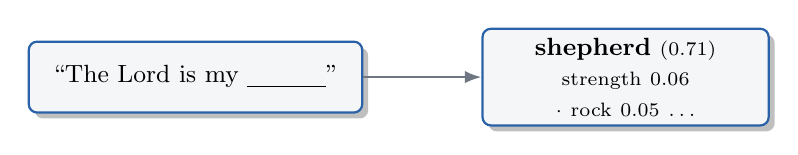
\begin{tikzpicture}[font=\small]
    \node[rectangle, rounded corners=3pt, draw=accentblue, thick, fill=lightgray, drop shadow,
          align=center, text width=4.0cm, minimum height=0.9cm] (ctx)
      {``The Lord is my \underline{\hspace{1.0cm}}''};
    \node[right=1.5cm of ctx, rectangle, rounded corners=3pt, draw=cAgent, thick, fill=lightgray,
          drop shadow, align=center, text width=3.4cm, minimum height=0.9cm] (pred)
      {\textbf{shepherd} \scriptsize(0.71)\\ \scriptsize strength 0.06 $\cdot$ rock 0.05 $\dots$};
    \draw[-{Latex[length=6pt]}, thick, midgray] (ctx)--(pred);
  \end{tikzpicture}
  \end{center}
  \vspace{2pt}
  \begin{center}\footnotesize\color{midgray}%
    It outputs a \emph{probability over every possible next token} --- then picks one, appends it, and repeats.\end{center}
  \vspace{6pt}
  \begin{columns}[t,totalwidth=\textwidth]
    \begin{column}{0.48\textwidth}
      \begin{featbox}{accentblue}{\faCogs\ What that means}
        \scriptsize It has no ``facts'' stored as facts. It has \textbf{patterns} of
        which words follow which --- learned from a huge amount of text.
      \end{featbox}
    \end{column}
    \begin{column}{0.04\textwidth}\end{column}
    \begin{column}{0.48\textwidth}
      \begin{featbox}{accentgold}{\faExclamationTriangle\ The consequence}
        \scriptsize It optimizes for \textbf{plausible}, not \textbf{true}. A fluent
        wrong answer scores as well as a right one \emph{to the model}.
      \end{featbox}
    \end{column}
  \end{columns}
  \vspace{6pt}
  \begin{center}\small\color{labnavy}Everything else today --- embeddings, temperature, hallucination --- follows from this one line.\end{center}
\end{frame}

% ---------------------------------------------------------------- tokens -> numbers
\begin{frame}{First it turns words into numbers: tokens \& embeddings}
  % --- compact pipeline spine ---
  \begin{center}
  
\begin{tikzpicture}[font=\scriptsize,
      b/.style={rectangle, rounded corners=3pt, draw, thick, fill=lightgray, drop shadow,
                align=center, text width=2.05cm, minimum height=0.72cm}]
    \node[b, draw=labnavy]    (txt)  {\textbf{Text}};
    \node[b, draw=accentteal, right=0.85cm of txt] (tok) {\textbf{Tokens}\\ \scriptsize integer IDs};
    \node[b, draw=accentblue, right=0.85cm of tok] (emb) {\textbf{Embeddings}\\ \scriptsize vectors};
    \node[b, draw=cAgent,   right=0.85cm of emb] (mdl) {\textbf{Model}\\ \scriptsize next token};
    \draw[-{Latex[length=5pt]}, thick, midgray] (txt)--(tok);
    \draw[-{Latex[length=5pt]}, thick, midgray] (tok)--(emb);
    \draw[-{Latex[length=5pt]}, thick, midgray] (emb)--(mdl);
  \end{tikzpicture}
  \end{center}
  \vspace{2pt}
  \begin{center}\scriptsize\color{midgray}%
    Real output of the \textbf{Meta-Llama-3.1-8B} tokenizer (128k vocab) --- the model you call on ALCF.\end{center}
  % --- example 1: a familiar phrase, ~one token per word ---
  {\scriptsize\color{labnavy}\bfseries A familiar phrase --- usually $\sim$one token per word (and the {\color{midgray}\textvisiblespace} space is \emph{part of} the token):}\\[2pt]
  \begin{center}
  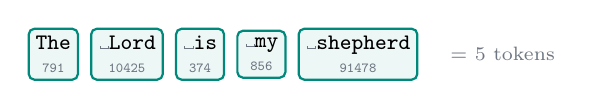
\begin{tikzpicture}[font=\ttfamily\footnotesize, node distance=4pt,
      chip/.style={rectangle, rounded corners=2pt, draw=cRAG, thick, fill=cRAG!7,
                   inner sep=2.5pt, align=center, minimum height=0.54cm, text depth=0pt}]
    \node[chip] (a1) {The\\[-1pt]{\tiny\color{midgray}791}};
    \node[chip, right=of a1] (a2) {{\color{midgray}\textvisiblespace}Lord\\[-1pt]{\tiny\color{midgray}10425}};
    \node[chip, right=of a2] (a3) {{\color{midgray}\textvisiblespace}is\\[-1pt]{\tiny\color{midgray}374}};
    \node[chip, right=of a3] (a4) {{\color{midgray}\textvisiblespace}my\\[-1pt]{\tiny\color{midgray}856}};
    \node[chip, right=of a4] (a5) {{\color{midgray}\textvisiblespace}shepherd\\[-1pt]{\tiny\color{midgray}91478}};
    \node[right=8pt of a5, font=\rmfamily\scriptsize\color{midgray}] {$=$ 5 tokens};
  \end{tikzpicture}
  \end{center}
  \vspace{2pt}
  % --- example 2: a proper name shatters into word-pieces ---
  {\scriptsize\color{labnavy}\bfseries A proper name shatters into \emph{word-pieces} --- and even ``grace'' is not one token:}\\[2pt]
  \begin{center}
  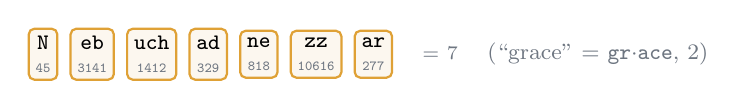
\begin{tikzpicture}[font=\ttfamily\footnotesize, node distance=4pt,
      chip/.style={rectangle, rounded corners=2pt, draw=accentgold, thick, fill=accentgold!8,
                   inner sep=2.5pt, align=center, minimum height=0.54cm, text depth=0pt}]
    \node[chip] (b1) {N\\[-1pt]{\tiny\color{midgray}45}};
    \node[chip, right=of b1] (b2) {eb\\[-1pt]{\tiny\color{midgray}3141}};
    \node[chip, right=of b2] (b3) {uch\\[-1pt]{\tiny\color{midgray}1412}};
    \node[chip, right=of b3] (b4) {ad\\[-1pt]{\tiny\color{midgray}329}};
    \node[chip, right=of b4] (b5) {ne\\[-1pt]{\tiny\color{midgray}818}};
    \node[chip, right=of b5] (b6) {zz\\[-1pt]{\tiny\color{midgray}10616}};
    \node[chip, right=of b6] (b7) {ar\\[-1pt]{\tiny\color{midgray}277}};
    \node[right=7pt of b7, font=\rmfamily\scriptsize\color{midgray}]
      {\rmfamily\scriptsize $=$ 7 \quad {\footnotesize(``grace'' $=$ \texttt{gr}$\cdot$\texttt{ace}, 2)}};
  \end{tikzpicture}
  \end{center}
  \vspace{2pt}
  \begin{center}\scriptsize\color{labnavy}%
    Each token then becomes an \textbf{embedding} (a vector) --- the hinge to Week 4, where retrieval \emph{is} ``find the nearest vectors.''\end{center}
\end{frame}

% ---------------------------------------------------------------- embeddings geometry
\begin{frame}{Meaning as geometry: why embeddings matter for us}
  \begin{columns}[c, totalwidth=\textwidth]
    \begin{column}{0.52\textwidth}
      \begin{center}
      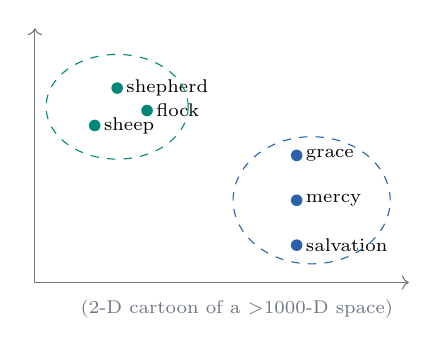
\begin{tikzpicture}[font=\scriptsize, scale=0.95, every node/.style={transform shape}]
        \draw[->, midgray] (0,0) -- (5.0,0);
        \draw[->, midgray] (0,0) -- (0,3.4);
        % cluster 1: shepherd / pastoral
        \fill[cRAG]   (1.1,2.6) circle (2.2pt) node[right,black]{shepherd};
        \fill[cRAG]   (0.8,2.1) circle (2.2pt) node[right,black]{sheep};
        \fill[cRAG]   (1.5,2.3) circle (2.2pt) node[right,black]{flock};
        \draw[cRAG, dashed] (1.1,2.35) ellipse (0.95cm and 0.7cm);
        % cluster 2: grace / salvation
        \fill[cAgent] (3.5,1.7) circle (2.2pt) node[right,black]{grace};
        \fill[cAgent] (3.5,1.1) circle (2.2pt) node[right,black]{mercy};
        \fill[cAgent] (3.5,0.5) circle (2.2pt) node[right,black]{salvation};
        \draw[cAgent, dashed] (3.7,1.1) ellipse (1.05cm and 0.85cm);
        \node[text=midgray] at (2.7,-0.35) {\scriptsize (2-D cartoon of a $>$1000-D space)};
      \end{tikzpicture}
      \end{center}
    \end{column}
    \begin{column}{0.46\textwidth}
      \small
      \begin{itemize}
        \item Related words land \textbf{near} each other --- the model learned this
          from usage, not a dictionary.
        \item ``Distance'' becomes something you can \textbf{compute}: cosine
          similarity between two vectors.
        \item Ask \emph{``which verses are closest to this question?''} and you get
          real passages back.
      \end{itemize}
      \vspace{2pt}
      {\scriptsize\color{midgray}That query is exactly what a RAG retriever does --- Week 4.}
    \end{column}
  \end{columns}
  \vspace{2pt}
  \begin{center}\small\color{labnavy}\bfseries Embeddings are how a machine ``measures'' meaning.\end{center}
\end{frame}

% ---------------------------------------------------------------- temperature
\begin{frame}{Same box, one knob: temperature}
  \begin{center}
  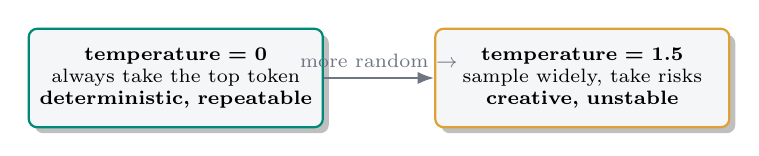
\begin{tikzpicture}[font=\scriptsize,
      b/.style={rectangle, rounded corners=3pt, draw, thick, fill=lightgray, drop shadow,
                align=center, text width=3.5cm, minimum height=1.25cm}]
    \node[b, draw=cRAG]    (lo)  {\textbf{temperature = 0}\\ \scriptsize always take the top token\\ \textbf{deterministic, repeatable}};
    \node[b, draw=accentgold, right=1.4cm of lo] (hi) {\textbf{temperature = 1.5}\\ \scriptsize sample widely, take risks\\ \textbf{creative, unstable}};
    \draw[-{Latex[length=6pt]}, thick, midgray] (lo)--(hi) node[midway,above,font=\scriptsize,text=midgray]{more random $\rightarrow$};
  \end{tikzpicture}
  \end{center}
  \vspace{8pt}
  \begin{center}
  \begin{minipage}{0.9\textwidth}\small
    The model always produces a probability distribution. \textbf{Temperature} controls
    how boldly you sample from it: near 0 you get the safe, reproducible answer; high,
    you get variety --- and more chances to go off the rails.
  \end{minipage}
  \end{center}
  \vspace{8pt}
  \begin{center}\small\color{labnavy}\bfseries
    For scholarship you usually want \emph{low} temperature --- and you \emph{report} the number.\end{center}
\end{frame}

% ---------------------------------------------------------------- hallucination (the money slide)
\begin{frame}{The money moment: confident, fluent, and wrong}
  \vspace{2pt}
  \begin{calloutbox}[accentgold]
    \large\faExclamationTriangle\ \textbf{Ask a small model for an obscure or
    made-up verse --- it will invent one, in flawless biblical cadence.}
  \end{calloutbox}
  \vspace{10pt}
  \begin{columns}[t, totalwidth=\textwidth]
    \begin{column}{0.48\textwidth}
      \begin{featbox}{accentgold}{\faQuestionCircle\ Why it happens}
        \scriptsize It is completing a \textbf{pattern}, not looking something up.
        ``A verse citation'' has a shape; it fills the shape convincingly whether or
        not the verse exists.
      \end{featbox}
    \end{column}
    \begin{column}{0.04\textwidth}\end{column}
    \begin{column}{0.48\textwidth}
      \begin{featbox}{cRAG}{\faUserShield\ What fixes it}
        \scriptsize Don't ask it to \emph{recall} --- give it the \textbf{real text}
        and ask it to \emph{use} that. Grounding = \textbf{RAG} (Wk 4). Checking =
        \textbf{evaluation} (Wk 6).
      \end{featbox}
    \end{column}
  \end{columns}
  \vspace{8pt}
  \begin{center}\small\color{labnavy}%
    In theology a fabricated reference is a \textbf{scholarly and pastoral failure}. You will reproduce this live today --- so you never forget it.\end{center}
\end{frame}

% ---------------------------------------------------------------- LLM to agent (four additions)
\begin{frame}{So what turns this predictor into an \emph{agent}?}
  \begin{center}\small
  On its own the model answers once and stops. Add four things and it can
  \textbf{pursue a goal}:
  \end{center}
  \vspace{4pt}
  \begin{columns}[t, totalwidth=\textwidth]
    \begin{column}{0.235\textwidth}
      \begin{featbox}{cAgent}{\faTools\ Tools}
        \scriptsize Call a retriever, a calculator, a code runner, the web ---
        \textbf{reach outside itself}.
      \end{featbox}
    \end{column}
    \begin{column}{0.02\textwidth}\end{column}
    \begin{column}{0.235\textwidth}
      \begin{featbox}{cRAG}{\faBrain\ Memory}
        \scriptsize Carry state across steps --- what it found, what it decided.
      \end{featbox}
    \end{column}
    \begin{column}{0.02\textwidth}\end{column}
    \begin{column}{0.235\textwidth}
      \begin{featbox}{accentblue}{\faSync\ Plan--act--observe}
        \scriptsize Decompose, act, \emph{look at the result}, decide the next step.
      \end{featbox}
    \end{column}
    \begin{column}{0.02\textwidth}\end{column}
    \begin{column}{0.235\textwidth}
      \begin{featbox}{cEval}{\faCompass\ Autonomy}
        \scriptsize Run many steps toward a goal without a human at each one.
      \end{featbox}
    \end{column}
  \end{columns}
  \vspace{10pt}
  \begin{center}\small\color{labnavy}%
    The model you talk to today is the \textbf{engine}. An agent is that engine \emph{plus a loop}.\end{center}
\end{frame}

% ---------------------------------------------------------------- the loop
\begin{frame}{The loop: plan $\to$ act $\to$ observe $\to$ repeat}
  \begin{center}
  \begin{tikzpicture}[font=\small,
      node distance=0.95cm and 1.7cm,
      stg/.style={rectangle, rounded corners=3pt, draw, thick, fill=lightgray,
                  drop shadow, align=center, text width=1.9cm, minimum height=0.9cm}]
    \node[stg, draw=labnavy]  (goal)    {\faBullseye\\ Goal};
    \node[stg, draw=cAgent, right=of goal] (plan) {\faSitemap\\ Plan};
    \node[stg, draw=cRAG, right=of plan]   (act)  {\faTools\\ Act\\ \scriptsize(call a tool)};
    \node[stg, draw=accentblue, right=of act] (obs) {\faEye\\ Observe\\ \scriptsize(read result)};
    \node[stg, draw=cEval, below=of act] (ans) {\faCheckDouble\\ Answer\\ \scriptsize(with citation)};
    \draw[-{Latex[length=6pt]}, thick, midgray] (goal) -- (plan);
    \draw[-{Latex[length=6pt]}, thick, midgray] (plan) -- (act);
    \draw[-{Latex[length=6pt]}, thick, midgray] (act)  -- (obs);
    \draw[-{Latex[length=6pt]}, thick, midgray] (obs.south) to[out=-90,in=0] node[right,font=\scriptsize,text width=1.6cm]{reflect \& loop} (act.east |- ans.east) -- (ans.east);
    \draw[-{Latex[length=6pt]}, thick, cAgent] (obs) to[out=120,in=60] node[above,font=\scriptsize]{not done?} (plan);
  \end{tikzpicture}
  \end{center}
  \vspace{4pt}
  \begin{center}\small\color{midgray}%
    Today we isolate the very first box --- the raw \emph{Act$\to$Observe} on one model call.\end{center}
\end{frame}

% ---------------------------------------------------------------- why open weights / why ALCF
\begin{frame}{Why an \emph{open} model, and why on ALCF}
  \begin{columns}[t, totalwidth=\textwidth]
    \begin{column}{0.31\textwidth}
      \begin{featbox}{cEval}{\faClipboardCheck\ Reproducible}
        \scriptsize ``Llama-3.1-8B, temp\,=\,0, ALCF'' is a \textbf{disclosable}
        fact. ``ChatGPT, last spring'' is not. Your appendix needs the former.
      \end{featbox}
    \end{column}
    \begin{column}{0.035\textwidth}\end{column}
    \begin{column}{0.31\textwidth}
      \begin{featbox}{cRAG}{\faLock\ Governed}
        \scriptsize A licensed translation or private corpus \textbf{stays on ALCF} ---
        it never leaves for a vendor. Matters once we load your texts (Wk 3).
      \end{featbox}
    \end{column}
    \begin{column}{0.035\textwidth}\end{column}
    \begin{column}{0.31\textwidth}
      \begin{featbox}{cAgent}{\faKey\ Yours}
        \scriptsize Free with your ALCF account --- no personal API keys on shared
        machines, and the \textbf{same client all term}.
      \end{featbox}
    \end{column}
  \end{columns}
  \vspace{12pt}
  \begin{center}
  \begin{minipage}{0.9\textwidth}\small
    The endpoint is \textbf{OpenAI-compatible}: the $\sim$15 lines you write today become
    the \emph{retriever's brain} in Week 4, unchanged. One model client, one corpus, one
    agent --- all term.
  \end{minipage}
  \end{center}
\end{frame}

% ================================================================ PART 2
\begin{frame}{Part 2 --- Hands-on: talk to the model directly}
  \vspace{2pt}
  \begin{calloutbox}[accentteal]
    \small\faInfoCircle\ The \textbf{ALCF inference endpoint} serves open-weight models
    (Llama, Qwen, \dots) behind a simple web API. No cluster, no queue --- just
    \texttt{messages in $\to$ completion out}. This is the raw box from Part 1.
  \end{calloutbox}
  \vspace{8pt}
  \begin{center}
  \begin{tikzpicture}[font=\scriptsize,
      s/.style={rectangle, rounded corners=3pt, draw, thick, fill=lightgray,
                drop shadow, align=center, text width=2.5cm, minimum height=1.15cm}]
    \node[s, draw=accentblue] (a)   {\faKey\\ \textbf{1. Log in}\\ Globus browser flow};
    \node[s, draw=cRAG, right=1.1cm of a] (b) {\faList\\ \textbf{2. List models}\\ see what's served};
    \node[s, draw=cAgent, right=1.1cm of b] (c) {\faComments\\ \textbf{3. Ask it}\\ 15-line client};
    \node[s, draw=accentgold, right=1.1cm of c] (d) {\faFlask\\ \textbf{4. Experiment}\\ temp + hallucinate};
    \draw[-{Latex[length=5pt]}, thick, midgray] (a)--(b);
    \draw[-{Latex[length=5pt]}, thick, midgray] (b)--(c);
    \draw[-{Latex[length=5pt]}, thick, midgray] (c)--(d);
  \end{tikzpicture}
  \end{center}
  \vspace{4pt}
  \begin{center}\footnotesize\color{midgray}%
    Notebook + one-page handout are in the course materials: \texttt{tutorials/week02\_alcf\_inference/}.\end{center}
\end{frame}

% ---------------------------------------------------------------- step 1: auth
\begin{frame}[fragile]{Step 1 --- Authenticate (once, good for $\sim$48 hours)}
  \begin{columns}[t, totalwidth=\textwidth]
    \begin{column}{0.52\textwidth}
      {\footnotesize\bfseries\color{accentblue}\faKey\ Get the helper \& log in}
      \begin{lstlisting}[style=shell]
# one-time: grab the auth helper
wget https://raw.githubusercontent.com/\
argonne-lcf/inference-endpoints/main/\
inference_auth_token.py

# opens a browser: log in with ALCF/Globus
python inference_auth_token.py authenticate
      \end{lstlisting}
    \end{column}
    \begin{column}{0.48\textwidth}
      {\footnotesize\bfseries\color{cRAG}\faList\ See what models are served}
      \begin{lstlisting}[style=shell]
tok=$(python inference_auth_token.py \
      get_access_token)

curl -s https://inference-api.alcf.anl.gov/\
resource_server/list-endpoints \
  -H "Authorization: Bearer $tok"
      \end{lstlisting}
      {\scriptsize\color{midgray}Copy an exact model ID from this list --- you'll paste it next.}
    \end{column}
  \end{columns}
  \vspace{6pt}
  \begin{center}\footnotesize\color{midgray}%
    Token lasts $\sim$48\,h; re-run \texttt{authenticate} when calls start returning 401.\end{center}
\end{frame}

% ---------------------------------------------------------------- step 2: the client
\begin{frame}[fragile]{Step 2 --- The 15 lines that carry the whole term}
  \begin{lstlisting}[style=shell, title=Python (OpenAI-compatible client)]
from openai import OpenAI
from inference_auth_token import get_access_token

client = OpenAI(
    api_key=get_access_token(),
    base_url="https://inference-api.alcf.anl.gov/resource_server/sophia/vllm/v1",
)

resp = client.chat.completions.create(
    model="meta-llama/Meta-Llama-3.1-8B-Instruct",   # use an ID from list-endpoints
    messages=[{"role": "user", "content": "What does Romans 7:24 say?"}],
    temperature=0,
)
print(resp.choices[0].message.content)
  \end{lstlisting}
  \begin{center}\footnotesize\color{midgray}%
    \texttt{pip install openai} first. Same call shape you'll reuse for retrieval and evaluation later.\end{center}
\end{frame}

% ---------------------------------------------------------------- step 3: the experiments
\begin{frame}{Step 3 --- Three tiny experiments, three big ideas}
  \begin{columns}[t, totalwidth=\textwidth]
    \begin{column}{0.31\textwidth}
      \begin{featbox}{cRAG}{\faThermometerHalf\ Temperature}
        \scriptsize Same prompt at \texttt{temp=0} twice (identical) vs \texttt{temp=1.5}
        three times (all different). \textbf{See determinism vs.\ sampling.}
      \end{featbox}
    \end{column}
    \begin{column}{0.035\textwidth}\end{column}
    \begin{column}{0.31\textwidth}
      \begin{featbox}{accentgold}{\faGhost\ Hallucination}
        \scriptsize Ask for \emph{``Hezekiah 3:16''} (no such book). Watch it
        confidently produce a verse. \textbf{This is the lesson.}
      \end{featbox}
    \end{column}
    \begin{column}{0.035\textwidth}\end{column}
    \begin{column}{0.31\textwidth}
      \begin{featbox}{cAgent}{\faVectorSquare\ Grounding teaser}
        \scriptsize Paste the \emph{real} verse into the prompt and ask again ---
        the answer snaps to truth. \textbf{That's RAG, by hand.}
      \end{featbox}
    \end{column}
  \end{columns}
  \vspace{12pt}
  \begin{center}
  \begin{minipage}{0.9\textwidth}\small
    Each is a few lines in the notebook. The arc: the box is \textbf{creative}
    (temperature), \textbf{unreliable alone} (hallucination), and \textbf{trustworthy
    when grounded} (teaser) --- which is the whole course in miniature.
  \end{minipage}
  \end{center}
\end{frame}

% ================================================================ RAG mini-section (capstone / preview of Week 4)
\begin{frame}{From teaser to method: this is RAG}
  \begin{center}\small
  You just grounded \emph{one} verse by hand. \textbf{RAG} automates that: for any
  question, first \emph{find} the right passages, then answer \emph{only} from them.
  \end{center}
  \vspace{6pt}
  \begin{center}
  \begin{tikzpicture}[font=\scriptsize,
      s/.style={rectangle, rounded corners=3pt, draw, thick, fill=lightgray,
                drop shadow, align=center, text width=2.3cm, minimum height=1.15cm}]
    \node[s, draw=labnavy]    (q)  {\faQuestionCircle\\ \textbf{Question}\\ \scriptsize ``body of death?''};
    \node[s, draw=cRAG, right=0.95cm of q] (r) {\faSearch\\ \textbf{Retrieve}\\ \scriptsize nearest verses};
    \node[s, draw=accentblue, right=0.95cm of r] (g) {\faLayerGroup\\ \textbf{Ground}\\ \scriptsize verses $\to$ prompt};
    \node[s, draw=cAgent, right=0.95cm of g] (a) {\faComments\\ \textbf{Generate}\\ \scriptsize cited answer};
    \draw[-{Latex[length=5pt]}, thick, midgray] (q)--(r);
    \draw[-{Latex[length=5pt]}, thick, midgray] (r)--(g);
    \draw[-{Latex[length=5pt]}, thick, midgray] (g)--(a);
    \node[below=0.45cm of r, text width=3.0cm, align=center, font=\scriptsize, text=midgray]
      {from \emph{your} corpus\\(all 31{,}100 KJV verses)};
  \end{tikzpicture}
  \end{center}
  \vspace{2pt}
  \begin{columns}[t, totalwidth=\textwidth]
    \begin{column}{0.48\textwidth}
      \begin{featbox}{cRAG}{\faKey\ The one rule}
        \scriptsize The model may use \textbf{only} the retrieved text. If the answer
        isn't there, it must \textbf{say so} --- not invent.
      \end{featbox}
    \end{column}
    \begin{column}{0.04\textwidth}\end{column}
    \begin{column}{0.48\textwidth}
      \begin{featbox}{accentblue}{\faSync\ Same client}
        \scriptsize Retrieve \emph{and} generate both call the \textbf{same} ALCF
        endpoint from Step 2 --- no new tools.
      \end{featbox}
    \end{column}
  \end{columns}
\end{frame}

% ---------------------------------------------------------------- RAG: with vs without on the whole Bible
\begin{frame}{RAG on the whole Bible: with vs.\ without}
  \begin{columns}[t, totalwidth=\textwidth]
    \begin{column}{0.48\textwidth}
      \begin{featbox}{accentgold}{\faGhost\ WITHOUT RAG --- from memory}
        \scriptsize A small model \textbf{paraphrases} Scripture and \textbf{invents}
        chapter:verse. Fluent, familiar-sounding --- and often subtly \textbf{wrong}.
        \\[4pt]{\tiny\color{midgray}\emph{``Hezekiah 3:16''} $\to$ a confident, fabricated verse.}
      \end{featbox}
    \end{column}
    \begin{column}{0.04\textwidth}\end{column}
    \begin{column}{0.48\textwidth}
      \begin{featbox}{cRAG}{\faCheckDouble\ WITH RAG --- from the text}
        \scriptsize Retrieves from all \textbf{31,100 verses}, quotes \textbf{exactly},
        and \textbf{cites}. Ask for a book that doesn't exist and it \textbf{declines}.
        \\[4pt]{\tiny\color{midgray}\emph{``Hezekiah 3:16''} $\to$ ``Not found in the provided verses.''}
      \end{featbox}
    \end{column}
  \end{columns}
  \vspace{8pt}
  \begin{calloutbox}[cRAG]
    \small\faBalanceScale\ \textbf{The theological stakes:} a paraphrase can drift
    doctrine; an exact citation can be \textbf{checked}. RAG turns the model from a
    \emph{source} into a \emph{finder} --- the scholar stays in charge of the text.
  \end{calloutbox}
  \vspace{2pt}
  \begin{center}\footnotesize\color{midgray}%
    Run it today: \texttt{bible\_rag/ask\_bible.py} --- same question, both ways.\end{center}
\end{frame}

% ---------------------------------------------------------------- RAG: how retrieval finds it
\begin{frame}{How it finds the verse: words now, meaning next}
  \begin{columns}[t, totalwidth=\textwidth]
    \begin{column}{0.48\textwidth}
      \begin{featbox}{accentblue}{\faSearch\ Keyword match (today)}
        \scriptsize \textbf{BM25}: rank verses by shared words. Pure Python, instant
        over 31k verses, no setup. Nails phrases (\emph{``still small voice''}) and
        citations.
      \end{featbox}
    \end{column}
    \begin{column}{0.04\textwidth}\end{column}
    \begin{column}{0.48\textwidth}
      \begin{featbox}{cRAG}{\faVectorSquare\ Meaning match (next)}
        \scriptsize \textbf{Embeddings}: rank by \emph{nearest vectors} --- Slide 6's
        geometry. Catches paraphrase (\emph{``the greatest commandment''}) that shares
        no keywords.
      \end{featbox}
    \end{column}
  \end{columns}
  \vspace{8pt}
  \begin{center}
  \begin{minipage}{0.9\textwidth}\small
    Same \textbf{retrieve $\to$ ground $\to$ generate} loop --- only the \emph{ranking}
    step changes. The lab ships with keyword search working out of the box;
    \texttt{build\_index.py} adds the embedding upgrade.
  \end{minipage}
  \end{center}
  \vspace{4pt}
  \begin{center}\small\color{labnavy}\bfseries%
    Retrieval is the bridge from Slide 6's ``meaning as geometry'' to a cited answer.\end{center}
\end{frame}

% ================================================================ touchpoint / wrap
\begin{frame}{Project touchpoint (20 min): point the box at \emph{your} question}
  \setlength{\leftmargini}{16pt}
  \begin{itemize}\small
    \item Take the \textbf{interest statement} you wrote for Week 1. Turn it into
      \textbf{one factual question} an 8B model could plausibly get wrong.
    \item Run it at \texttt{temp=0}. \textbf{Fact-check the answer yourself.} Note
      exactly where it was fluent-but-wrong.
    \item That failing question is a \textbf{seed for your evaluation set} (Week 6) ---
      keep it.
  \end{itemize}
  \vspace{6pt}
  \begin{calloutbox}[cRAG]
    \small\faLightbulb\ \textbf{The through-line:} today you saw \emph{why} we need
    grounding and evaluation. Week 3 loads your corpus; Week 4 turns this same client
    into a retriever over it.
  \end{calloutbox}
\end{frame}

% ---------------------------------------------------------------- assignment
\begin{frame}{Assignment for next week}
  \begin{featbox}{accentblue}{\faFlask\ 1. Run it and save a trace}
    \small
    Get one real completion back from the ALCF endpoint. Save \textbf{one screenshot
    or transcript} of a hallucination you provoked --- model ID, temperature, prompt,
    and the wrong output. (This is your first disclosure-appendix artifact.)
  \end{featbox}
  \vspace{7pt}
  \begin{featbox}{accentteal}{\faBookOpen\ 2. Reading}
    \small
    \begin{itemize}
      \item Anthropic, \emph{Building Effective Agents} (2024) --- skim; note the
        tool-use loop.
      \item Weng, \emph{LLM-Powered Autonomous Agents} (2023) --- read the
        ``planning'' and ``memory'' sections.
      \item Optional: Wolfram, \emph{What Is ChatGPT Doing\dots?} --- the next-token section.
    \end{itemize}
  \end{featbox}
  \vspace{6pt}
  \begin{center}\small\color{labnavy}\bfseries
    Next week: the theological corpus --- the texts \emph{you} will ground on all term.\end{center}
\end{frame}

\end{document}
